\chapter{Results}
The following structure corresponds to the project instructions.

% Example: insert image
% \includegraphics{fig/NameOfTheFileWithoutExtension}

\section{Load VTK files and make the basic menu} 

\textbf{Header information from VTK file.}

\begin{table}[h]
	\ttfamily
	\small
	\begin{tabular}{l|l}
		1 & \# vtk DataFile Version 3.0     \\
		2 & vtk output                      \\
		3 & ASCII                           \\
		4 & DATASET STRUCTURED\_POINTS      \\
		& DIMENSIONS 256 256 230          \\
		& SPACING 1 1 1                   \\
		& ORIGIN 0 0 0                    \\
		5 & POINT\_DATA 15073280            \\
		& SCALARS scalars unsigned\_short \\
		& LOOKUP\_TABLE default          
	\end{tabular}
\end{table}

\noindent
\textbf{1} File version and identifier.\\
\textbf{2} Character string header terminated with \textbackslash n (max. 256 characters).\\
\textbf{3} File format: ASCII or BINARY.\\
\textbf{4} Dataset structure describing the geometry and topology of the dataset. Available structures: STRUCTURED\_POINTS, STRUCTURED\_GRID, UNSTRUCTURED\_GRID, POLYDATA, RECTILINEAR\_GRID, FIELD.\\
\textbf{5} Dataset attributes, number of data items = number of points in the dataset; dimension x*y*z = POINT\_DATA

The data in the given files is compressed by means of storing a single grayscale value for each point. Apart from this, no futher compression to file is applied.

\section{Planes for different views}

\begin{figure}
	\centering
	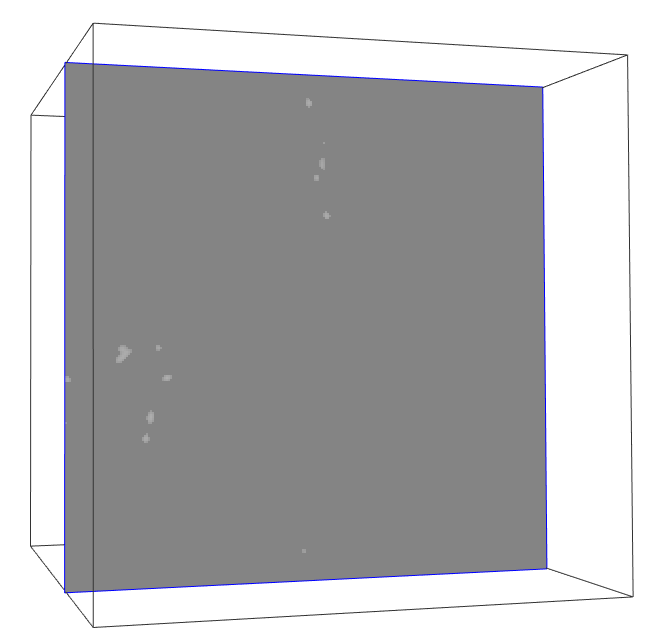
\includegraphics[scale=0.3]{fig/image-plane}
	\caption{Coronal view for segmented image.}
	\label{fig:image-plane}
\end{figure}

A class vtkImagePlaneWidget was used to show the cut from the segmented data (Figure \ref{fig:image-plane}). In segmented image view we can show sagittal, transversal and coronal views by pressing S, T and C keys respectively. The segmented image is then hidden in order to show a cut and scrolling through the slices is possible by pressing + and - keys.

\section{Marching cubes and building the skeleton}

\begin{figure}
	\centering
	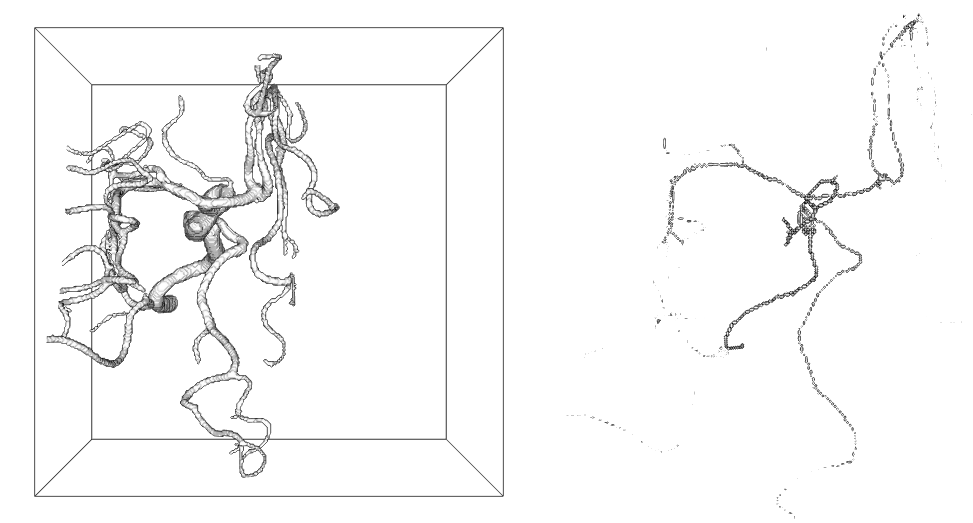
\includegraphics[scale=0.6]{fig/segmented-skeleton}
	\caption{vtkContourFilter used to render segmented and skeleton images.}
	\label{fig:segmented-skeleton}
\end{figure}

\begin{figure}
	\centering
	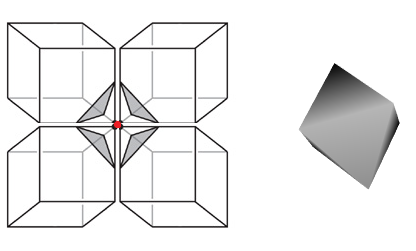
\includegraphics[scale=0.6]{fig/marching-cubes-1-point}
	\caption{Only one voxel with non-zero value (all other voxels are set to 0.)}
	\label{fig:marching-cubes-1-point}
\end{figure}

\begin{figure}
	\centering
	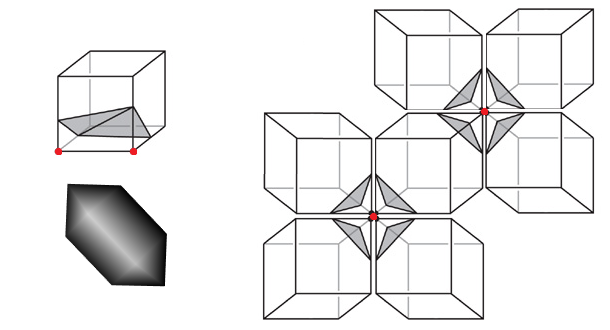
\includegraphics[scale=0.6]{fig/marching-cubes-2-points}
	\caption{Two voxels with non-zero value (all other voxels are set to 0.)}
	\label{fig:marching-cubes-2-points}
\end{figure}

% label doesn't work :/
\begin{lstlisting}[caption={A sample from skeleton file},label={lst:sample-skeleton}]
0 0 0 0 0 0 0 0 0 
0 0 0 0 0 0 14 0 0 
0 0 0 0 0 0 0 0 0 
\end{lstlisting}

A class vtkContourFilter was used to render segmented and skeleton images as they are in provided files (Figure \ref{fig:segmented-skeleton}).
The visualized skeleton path is not continuous due to provided data that was processed by vtkContourFilter. The values occur alone, the adjacent ones have value zero (Listing 1.1). If this situation occurs, there is a small cube mesh built around this voxel (Figure \ref{fig:marching-cubes-1-point}). Similar case is with two voxels with non-zero value (Figure \ref{fig:marching-cubes-2-points}).

TODO : -	Build the skeleton using the vtkTubeFilter (single tube should be used for a single branch. A branch in the skeleton image consists of neighboring voxels that have 2 neighbors (they are part of the path), and start and end voxel (they have either 1 or mode than 2 neighbors in their 3D neighborhood). In order to make a tube, the voxels have to be entered in a SEQUENTIAL order from one (start) voxel to the other (end) voxel).\\
-	How does the skeleton look like? Are the branches smooth? Why?\\
-	Make the branches smooth.\\

The tube filter generates a tube around each input line. Therefore we made lines between each of the neighboring voxels in the image. First we had to find each voxel, and connect them branch by branch. Next comes a description of our algorithm to solve that problem.

The algorithm of making polydata out of the skeleton image data is mainly done in 4 steps.
\begin{itemize}

\item Find first a voxel of the image, by greedily searching though the image voxel by voxel. Every voxel has a scalar value x, where x = 0 means that the voxel is not part of the image and x > 0, means that it is. 

\item Then find the end of the branch of that voxel. This is done by travelling from neighbor to neighbor until an end of the branch is found. In the search for neighbors of one voxel, the 26 surrounding voxels is investigated. Only unvisited neighbors are considered.

\item Starting with the end of the branch, the complete branch is found, while marking every found voxel visited. An end of a branch has either one neighbor or more than two neighbors. When an end that has more than two neighbors is found, the unvisited neighbors are saved to a stack S.

\item Take a voxel from stack S and repeat step 3. If S is empty, go to step 1. The algorithm finishes when the search at step 1 reaches the last voxel of the image.

\end{itemize}

After the search, polydata is made by making a polyline for each branch, making a point for each voxel and finally also add the voxel scalars to the polydata. The vtkTubeFilter can then be used to generate a tube around each polyline. This results in a skeleton that is not smooth. That is, the tubed skeleton forms a zick-zack pattern. We believe that the amount of points were too few for making it smooth. \\

To make the branches smooth we increased the number of polylines in the skeleton stucture with the vtkSplineFilter, which uniformly divides each line into several lines. Lines which have coincidental points are ignored by the spline filter, so to avoid that problem those coincidental points are removed by filtering the data through the vtkCleanPolyData filter. \\

If the scalars have been added to the polydata, making the radii and color vary by the scalar value of each voxel are simply done by two function calls (vtkTubeFilter::SetVaryRadiusToVaryRadiusByScalar(), vtkPolyDataMapper::ScalarVisibilityOn())

\section{Volume visualization}

\begin{figure}
	\centering
	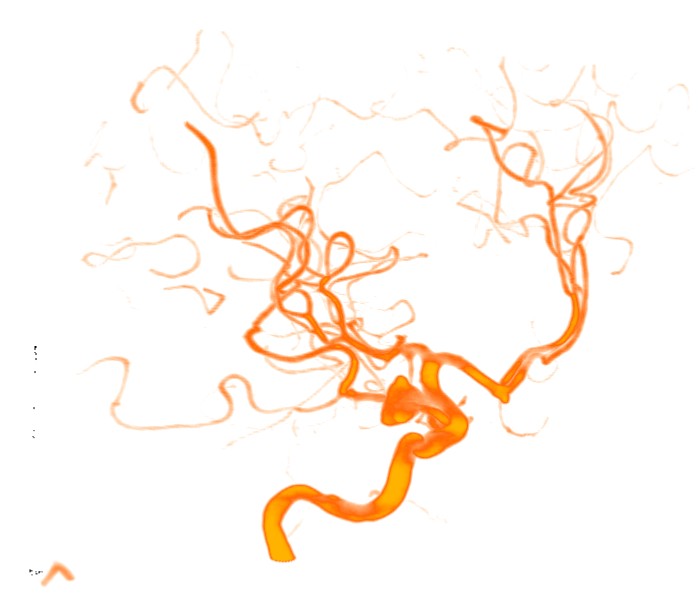
\includegraphics[scale=0.4]{fig/volume-rendering}
	\caption{Volume rendering.}
	\label{fig:volume-rendering}
\end{figure}

The volume visualization was obtained by using vtkVolumeRayCastMapper with vessels\_data.vtk (Figure \ref{fig:volume-rendering}). The crucial part was to set proper RGB points in vtkColorTransferFunction which correspond to luminance values from the VTK file.

Because it is very demanding to do volume visualization it can be useful to change the level of detail (LOD). \\
We first tried to add a vtkLODActor to the renderer. We set the low- and medium resolution filters of the LODActor, so that the actor would take care of the level of detail automatically as we changed the update rate of the render window interactor. vtkOutlineFilter as a low resolution filter and vtkMaskPoints as a medium resolution filter as were the default filters according to the VTK API. But as we noticed that we could simply change the level of detail with a single function call to the render window interactor without adding a LODActor, we used that functionality instead. There are two function calls to the render window interactor to have in mind here. vtkRenderWindowInteractor::SetDesiredUpdateRate(rate) controls the
update rate when the camera is used to rotated or zoom in on the image. The default value of this rate is 15 frames/second.
vtkRenderWindowInteractor::SetStillUpdateRate(rate) is for the update rate when the movement has stopped. When doing the volume rendering there could be a considerable difference in speed when using these two functions, especially if your computer is of an older model.

\section{Point picker and distance calculation}


\section{Visualization}


\section{Using the Spline Widget}

